\documentclass{article}
\usepackage{fullpage}
\usepackage{lastpage}
\usepackage{fancyhdr}
\usepackage{amssymb}
\usepackage{amsmath}
\usepackage{graphicx,subcaption} 
\usepackage{mathtools}
\usepackage{enumerate}
\usepackage{xspace}
\usepackage{txfonts}
\usepackage[citestyle=numeric]{biblatex}
\begin{document}
\begin{center}
{\Large \textbf{CMPUT 605: Exploring Methods for Guiding Exploration in Learning to Play Hex}}
\end{center}
\section*{Introduction}
The aim of this project was initially to investigate a particular method for guiding exploration in the board-game Hex in order to facilitate learning of approximate win probabilities for each available move in a state using a deep convolutional neural network. This method was based on the idea that the goal of exploration should be to follow lines of play that maximally reduce the Bernoulli variance in the state win probability estimate (i.e. $P_w(1-P_w)$) . This initial goal was found to be seemingly infeasible (at least in the particular form which was investigated here). Therefore other methods of improving learning in the game of Hex were also investigated, including exploration guided by pseudo-counts and using information generated by an existing hex solver to guide the learning and exploration.

For brevity, throughout we will use the notation $x\leftsquigarrow y$ to denote a gradient descent update which modifies the parameters of $x$ in order to reduce $(x-y)^2$.

\section*{Exploration by Estimated Variance Reduction}
The first idea tried for guiding exploration was based on learning probability estimates for each move based on the assumption that each move being a win was an independent Bernoulli event with some initially unknown probability. Expanding from this the idea was to also learn an estimated reduction in state win probability variance that would result by taking each move, playing out the rest of the game to the end, and performing a full backup of all move probabilities discovered along the way.

let $Q(S,A)$ be our win probability (or action value) estimate for each action $A$ in a given state $S$. Ordinary ones-step Q-learning (for 2 player minimax games) performs updates of the form:
$$Q(S_t,A_t)\leftsquigarrow 1-\max_A Q(S_{t+1},A)$$
In order to iteratively improve the estimated action values. Notice that if the game were stochastic and $Q(S_t,A_t)$ was equal to the true win probability, this update would be at a fixed point hence in case of stochastic games it makes some sense to say that $Q(S_t,A_t)$ is our estimate of the true winning probability of each move. Hex on the other hand is deterministic so each move has a true win probability of either 1 or 0, hence it is perhaps less clear what intermediate values of $Q(S_t,A_t)$ imply, however it can be roughly thought of as our degree of belief about the state being a win.

Given this interpretation we suggest an alternative update rule that makes this idea somewhat more explicit, and which will allow us to formulate the concept of state value variance reduction resulting from each particular move. Our new update rule assumes each move independently has a true value of either a win or a loss and therefore to do one step backups we look at the joint probability over the next state's moves as follows:
$$Q(S_t,A_t)\leftsquigarrow \prod_A 1-Q(S_{t+1},A)$$
i.e. the probability that the last move was a win should be the joint probability that every move in the resulting state is a loss for the opponent.

With this new formulation in mind we can get a state win probability as the probability that any move in the state is a win (i.e. not every move is a loss):
$$V(S_t)=1-\prod_A 1-Q(S_t,A)$$
Furthermore we can formulate the variance in this state win probability and attempt to choose moves which seek to reduce this variance using a tree backup of a maximally variance reducing rollout to the end of the game. The state value variance is given by:
$$\prod_A Q(S_t,A)-\prod_A Q(S_t,A)^2$$
Or notion of optimal exploration is as follows: we wish to follow some sequence of actions to the end of the game such that if we perform full backups of the form $Q(S_t,A_t)\leftarrow \prod_A 1-Q(S_{t+1},A)$ the reduction in the variance of out current state value estimate $\prod_A Q(S_t,A)-\prod_A Q(S_t,A)^2$ will be maximal. To simplify the problem and allow us to learn an estimate of expected variance reduction via one step backups we make the assumption that the expected change in $Q(S_t,A)$ resulting from taking action A and then following this procedure is 0. This is quite hand-wavy and perhaps ill-motivated, however it makes some sense in light of the fact that if we were to attempt to learn this change using the same model we use to learn $Q(S_t,A)$ itself, we would expect it to quickly converge to 0 simply because the model is already attempting to learn $Q(S_t,A)$ via one step backups. If we \textit{could} learn the expectation of this change was something other than 0 we could simply add this expectation to the current value estimate in order to generate a more accurate estimate without actually performing the lookahead.

With this assumption then our task remains to estimate the change in $Q(S_t,A)^2$ along a sequence of actions aiming to maximize this change. More concretely, call this quantity:
$$\Delta \sigma(S_t,A_t) = E[\max_{A_{t+1}}E[\max_{A_{t+2}}...(Q(S_t,A_t)^2-\prod_A Q_{new}(S_t,A_t)^2)...]]$$
where $Q_{new}(S_t,A)$ represents the new value $Q(S_t,A)$ after backing up along the followed action sequence $(A_t,A_{t+1},...)$. Now note that:
\begin{align*}
Q_{new}(S_t,A) &=Q(S_t,A) \text{ for } A\neq A_1\\
Q_{new}(S_t,A_t) &=\prod_A 1-Q_{new}(S_{t+1},A)\\
Q_{new}(S_t,A_t)^2&=\prod_A 1-2Q_{new}(S_{t+1},A)+Q_{new}(S_{t+1},A)^2\\
\end{align*}
\begin{align*}
\Delta \sigma(S_t,A_t) &= E[\max_{A_{t+1}}E[\max_{A_{t+2}}...( Q(S_t,A_t)^2- Q_{new}(S_t,A_t)^2)...]]\\
&=E[\max_{A_{t+1}}E[\max_{A_{t+2}}...((Q(S_t,A_t)^2-(\prod_{A} (1-Q(S_{t+1},A))^2+(\prod_{A} (1-Q(S_{t+1},A))^2-Q_{new}(S_t,A_t)^2)...]]\\
\intertext{using our assumption that $E[Q_{new}(S_t,A_t)]=Q(S_t,A_t)$ and the expansion of $Q_{new}(S_t,A_t)^2$ noted above... }
&=E[\max_{A_{t+1}}E[\max_{A_{t+2}}...(Q(S_t,A_t)^2-\prod_{A} (1-Q(S_{t+1},A))^2+\prod_{A\neq{A_{t+1}}} (1-Q(S_{t+1},A))^2(Q(S_{t+1},A_{t+1})^2-Q_{new}(S_{t+1},A_{t+1})^2)...]]\\
&=E[\max_{A_{t+1}}E[\max_{A_{t+2}}...(Q(S_t,A_t)^2-\prod_{A} (1-Q(S_{t+1},A))^2+\prod_{A\neq{A_{t+1}}} (1-Q(S_{t+1},A))^2\Delta \sigma(S_{t+1},A_{t+1}))...]]\\
&=E[(Q(S_t,A_t)^2-\prod_{A} (1-Q(S_{t+1},A))^2+\max_{A_{t+1}}\prod_{A\neq{A_{t+1}}} (1-Q(S_{t+1},A))^2\Delta \sigma(S_{t+1},A_{t+1}))]
\end{align*}
We have derived a recursive formula which we can now use to specify the following update rule for an exploration score network:
$$Q_{exp}(S_t,A_t)\leftsquigarrow Q(S_t,A_t)^2-\prod_{A'} (1-Q(S_{t+1},A'))^2+\max_A\prod_{A'\neq A} (1-Q(S_{t+1},A'))^2Q_{eAxp}(S_{t+1},A)$$
And we can define an "exploration greedy action selection" by noting that our goal in choosing actions should be to reduce the variance in the current state value estimate by as much as possible:
$$A_t= \text{argmax}_A\prod_{A'\neq A}(1-Q(S_t,A))^2Q_{exp}(S_t,A)$$
During training the idea was to select actions using an epsilon greedy version of this metric while simultaneously updating both the $Q$ and $Q_{exp}$ networks which would share some number of lower layers. 

This was attempted, however the joint distribution based update rule for $Q$ was not found to be feasible for learning on reasonable sized boards and hence there was no real opportunity to even test the $Q_{exp}$ network, which relies on $Q$.  Testing on 5x5 showed that the backup method could learn to some degree as shown in figure \cite{5x5}. However even on 5x5 it was still qualitatively outperformed by ordinary Q-Learning and performance degraded very rapidly when scaling to larger boards. For these reasons we did not bother to proceed with more rigorous testing of this method at this time. The reason for the failure appears to be simply that the method gets quickly lost in noise, and on larger boards more moves means there is far more noise to get lost in. The backup rule is essentially very pessimistic because if there are a large number of moves with even a small winning chance in the next state it will conclude that a loss is likely because the opponent has so many possible wins. This issue could potentially be remedied with more sophisticated statistical techniques and may be worth examining further in the future.
\begin{figure}[!ht]
\centering
\begin{subfigure}[t]{.45\textwidth}
  \centering
      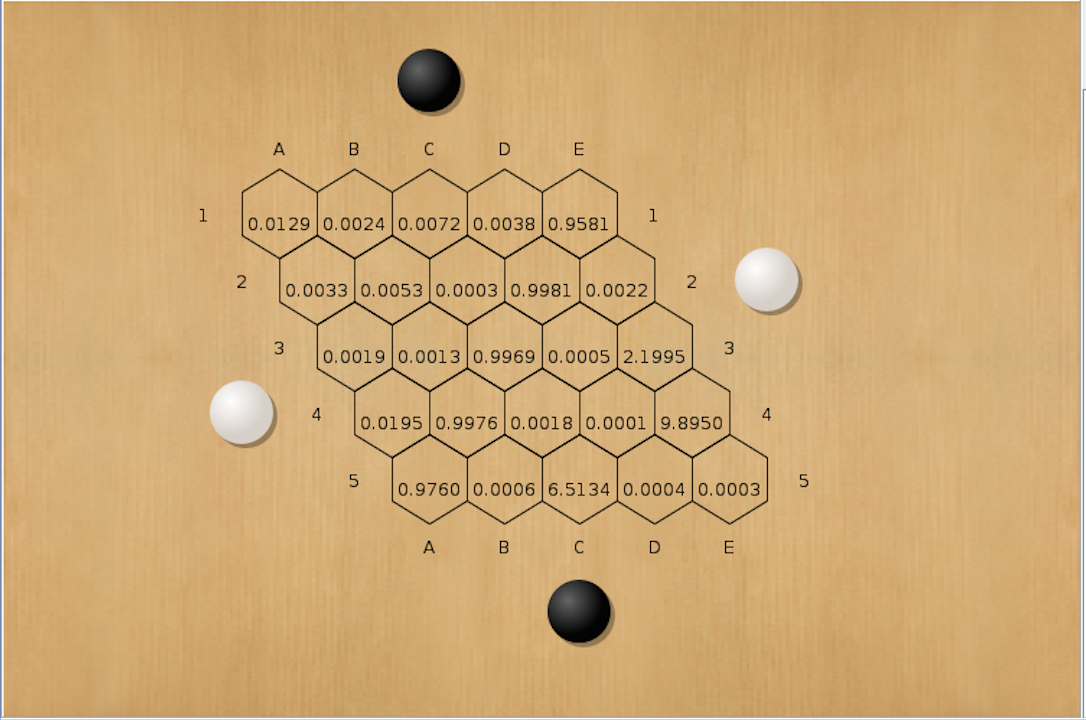
\includegraphics[width=1\textwidth]{pics/5x5_hex_opening.png}
  \caption{Scores for the 5x5 opening board learned using joint distribution backup. The scores close to 1 are in fact the only winning moves.}
  \label{fig:5x5_1}
\end{subfigure}\hfill
\begin{subfigure}[t]{.45\textwidth}
  \centering
      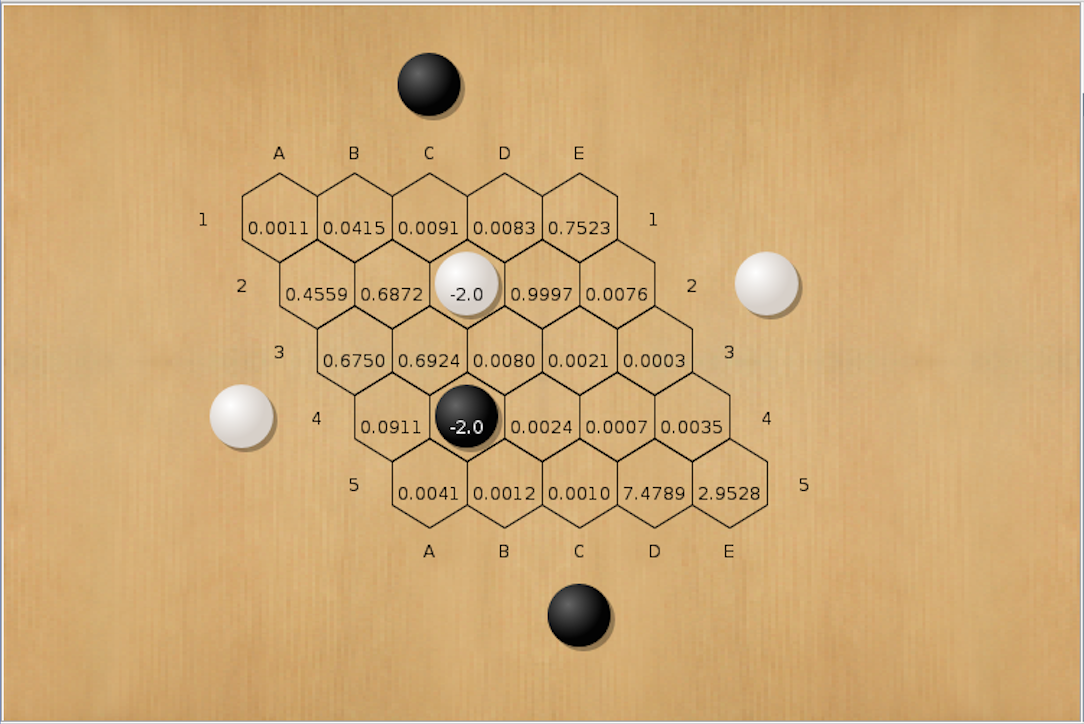
\includegraphics[width=1\textwidth]{pics/5x5_hex_2_moves.png}
  \caption{2 moves in, scores are still reasonable.}
  \label{fig:5x5_2}
\end{subfigure}
\caption{Expamples of 5x5 hexs scores learned by joint distribution backup rule. It scales very poorly to larger boards, but here it is adequate. Note, values  apparently greater than 1 are actually near 0 but the exponent was truncated.}
\label{fig:5x5}
\end{figure}


\section*{Pseudocount Exploration}
We also experimented with a second method for guiding exploration in Hex called pseudocount exploration, as highlighted in \cite{pseudocounts}. This method requires a learned model of probability for each experienced state which satisfies certain constraints outlined in \cite{pseudocounts}. Here we closely follow \cite{pseudocounts} and make use of the same Skip Context Tree Switching \cite{SCTS} model used there, in particular we make use of the python code available at \cite{SCTS_code}. This probability model is used to defined a "pseudocount" by analogy with the ordinary notion of count, which is itself associated with the empirical probabilities (i.e. visitation count for state s over total visitation count for all states).

We will now briefly discuss the notion of pseudocount and its motivation. Suppose we postulate (by analogy with ordinary count and total for the empirical distribution) for some arbitrary state probability model the existence of an associated pseudocount $N(x)$ and pseudocount total $n$. Note that for the empirical distribution the probabilities before and after visiting a state (say $p$ and $p'$) are related by:
$$p(x)=\frac{N(x)}{n},\ \ p'(x)=\frac{N(x)+1}{n+1}$$
Taking this as a defining property we can then solve for N(x) for an arbitrary probability distribution in terms of how the distribution is effected by the observation of state x.
$$N(x)=\frac{p(x)(1-p'(x))}{p'(x)-p(x)}$$
This pseudocount can then be used to give an added reward bonus for exploring less visited states. In \cite{pseudocounts} they use $\frac{\beta}{\sqrt{N(x)}}$ to generate the reward bonus for each state. In that work this reward bonus is simply added to the ordinary reward for each state and training proceeds by ordinary Q learning. In our case we had to modify this a bit because the game is adversarial, we require the value to be negated on each time-step to generate the opponent value, however we do not wish to negate the reward bonus. To allow us to do this we factor the value function into a true value and exploration value with updates done as follows:
$$Q(S_t,A_t) \leftarrow R(t) - Q(S_{t+1}, \text{argmax}_A(Q(S_{t+1}, A)+Q_{exp}(S_{t+1},A)))$$
$$Q_{exp}(S_t,A_t) \leftarrow R_{exp}(t) - Q(S_{t+1}, \text{argmax}_A(Q(S_{t+1}, A)+Q_{exp}(S_{t+1},A)))$$
Where $R(t)$ is the true reward, in this case simply win-loss, and $R_{exp}(t)=\frac{\beta}{\sqrt{N(x)}}$ is the exploration bonus. The networks for these two functions share all but the top few layers. We found $\beta=0.0025$ appeared to give a reasonable reward bonus in this case, we also found it necessary to restrict the action bonus to $(0,1)$ using a sigmoid at the output and apply a discount factor of $\gamma=0.95$ to prevent the exploration value from blowing up due to maximization over the large number of available actions.

This exploration method was primarily tested on the 7x7 board and did not yield any clear improvement over 100,000 training episodes. One possible reason is that the pseudo-count in its present form does a poor job of capturing the distribution of Hex states and so the pseudo-count really just serves to blur the values and slow learning. To give an example: one place pseudo-count exploration was shown to do particularly well was Montezuma's revenge which consists of a series of puzzle rooms with very sparse reward. The independent distinct rooms found in this game (and games like it) seem to provide a strong factored signal from the pseudo-count bonus reward. If a room has not been explored much, entering it, and remaining in it, will lead to large pseudo-count reward. If a room has been highly explored no such reward will be available. By contrast Hex has no such factored structure, each move results in a slight change to the state and thus the pseudo-counts will be highly diffuse and may not provide much of a meaningful signal. Perhaps what is needed to improve on this is a pseudo-count method which somehow incorporates meaningful generalization, rather than relying on a handcrafted probability model that works only under certain circumstances.

\section*{Integrating a Hex solver with the Learning Process}
This was not so much an exploration method, but another technique attempted to improve the learning of the network via providing additional information. Specifically the solver from benzene was integrated into the learner and used to limit move selection to the must-play region, as well as to find wins early and use the true value rather than 1-step Q-learning updates where possible. 

The must-play information was used simply by calling get-must-play in the solver before each move and choosing the highest value move over the must-play only whenever it was non-empty. When a random move was chosen (10\% chance currently) the learner could still play outside the must-play, this prevents overgeneralization to states outside the must-play, which if never tested may be learned to be similar to states within, which in general will be a very poor assumption. 

The solver information was more difficult to use because we did not want the learner to have to wait around for the solver to finish before proceeding on each move. In the end an asynchronous solution was used. The solver maintains a queue of moves made by the learner and is called on each move for a maximum time (currently set to 0.5s) while the learner proceeds. If the solver successfully solves a position or times out it checks to see if the queue remains under some threshold size (currently set to 50) if it does it will move on to solve the next position. If the queue grows above the maximum the solver will stop solving and simply play moves until the queue size is sufficiently reduced. Whenever a move is solved the solver modifies a value in the replay memory to indicate this and the learner uses this information to backup the true value rather than the one step Q-update whenever this memory is present in a future batch. 

This method was also tested on the 7x7 board and surprisingly also did not yield any clear improvement over 100,000 training episodes. Since both the must play and solver were integrated and tested together it is currently hard to say whether each of them may have been more effective individually. It is conceivable that integrating the must-play could have hurt performance since the pruned moves would end up being rarely played and may therefore have very inaccurate values leading them to be erroneously selected at test time. Integrating the must-play at test time as well would be one way to investigate this theory. It is also conceivable, though perhaps less likely that the addition of solver information itself could hurt performance. If the solver values are too far away from those learned by one step backup the learner may have difficulty actually working out the full strategy that allows it to find the wins indicated by the solver. The mixed information could pull the learner in two different directions so to speak and make learning more difficult. More testing is needed to make any reasonable conclusions here.

\section*{Results}
\begin{figure}[!ht]
\centering
\begin{subfigure}[t]{.45\textwidth}
  \centering
      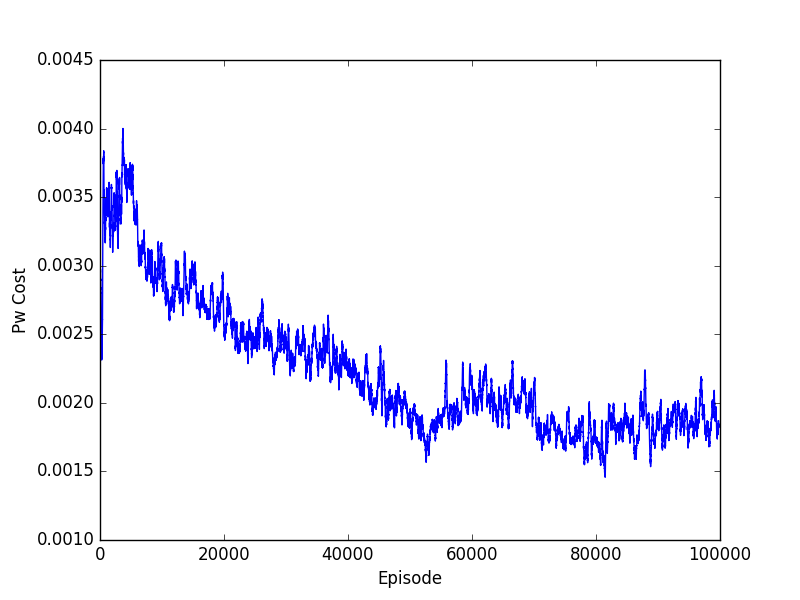
\includegraphics[width=1\textwidth]{pics/7x7_Q_Pw_cost.png}
  \caption{Scores for the 5x5 opening board learned using joint distribution backup. The scores close to 1 are in fact the only winning moves.}
  \label{fig:5x5_1}
\end{subfigure}\hfill
\begin{subfigure}[t]{.45\textwidth}
  \centering
      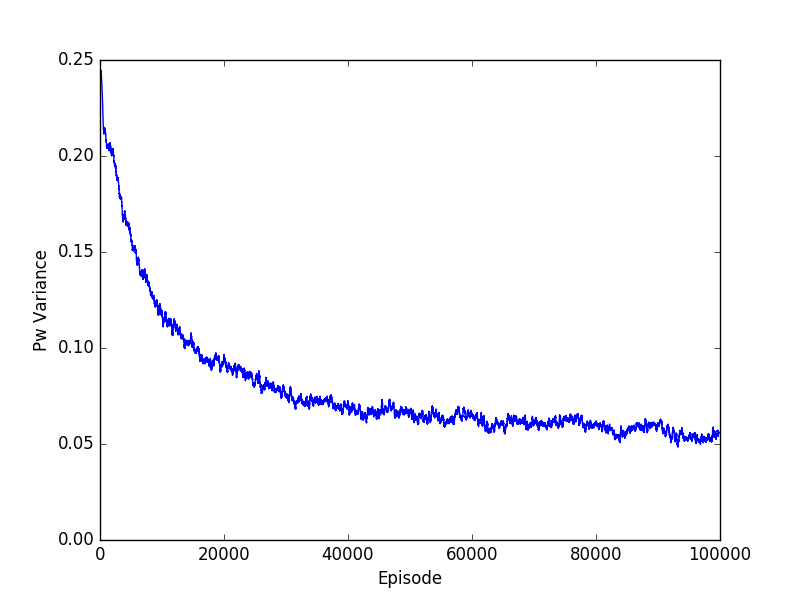
\includegraphics[width=1\textwidth]{pics/7x7_Q_Pw_var.png}
  \caption{2 moves in, scores are still reasonable.}
  \label{fig:5x5_2}
\end{subfigure}
\caption{Expamples of 5x5 hexs scores learned by joint distribution backup rule. It scales very poorly to larger boards, but here it is adequate. Note, values  apparently greater than 1 are actually near 0 but the exponent was truncated.}
\label{fig:5x5}
\end{figure}

\begin{figure}[!ht]
\centering
\begin{subfigure}[t]{.45\textwidth}
  \centering
      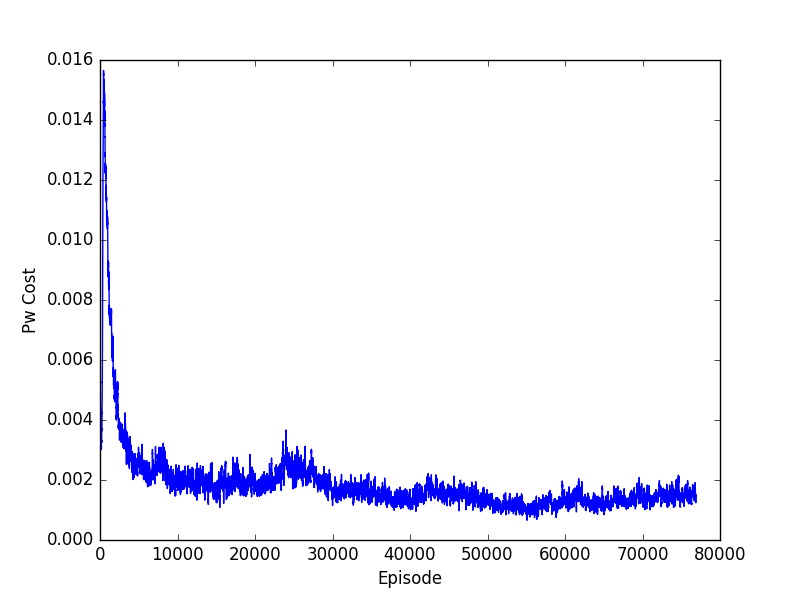
\includegraphics[width=1\textwidth]{pics/5x5_exp_Pw_cost.png}
  \caption{Scores for the 5x5 opening board learned using joint distribution backup. The scores close to 1 are in fact the only winning moves.}
  \label{fig:5x5_1}
\end{subfigure}\hfill
\begin{subfigure}[t]{.45\textwidth}
  \centering
      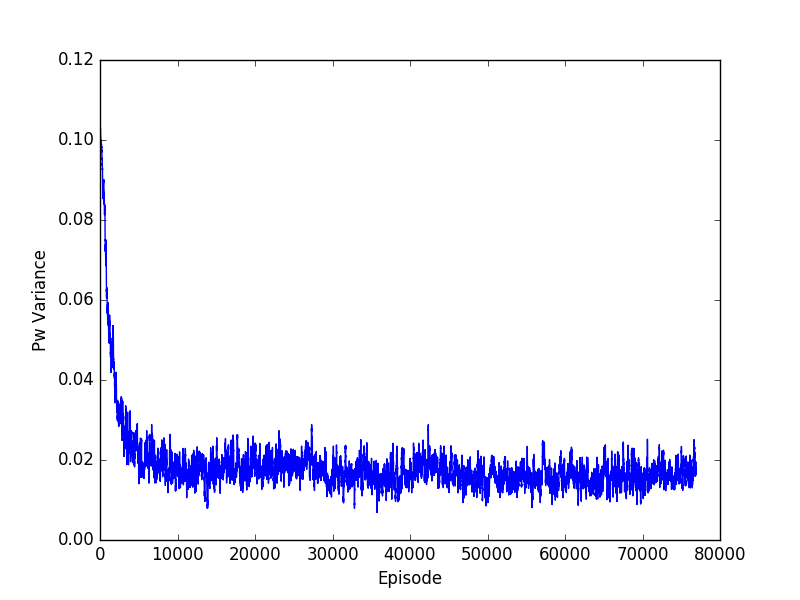
\includegraphics[width=1\textwidth]{pics/5x5_exp_Pw_var.png}
  \caption{2 moves in, scores are still reasonable.}
  \label{fig:5x5_2}
\end{subfigure}\vfill
\begin{subfigure}[t]{.45\textwidth}
  \centering
      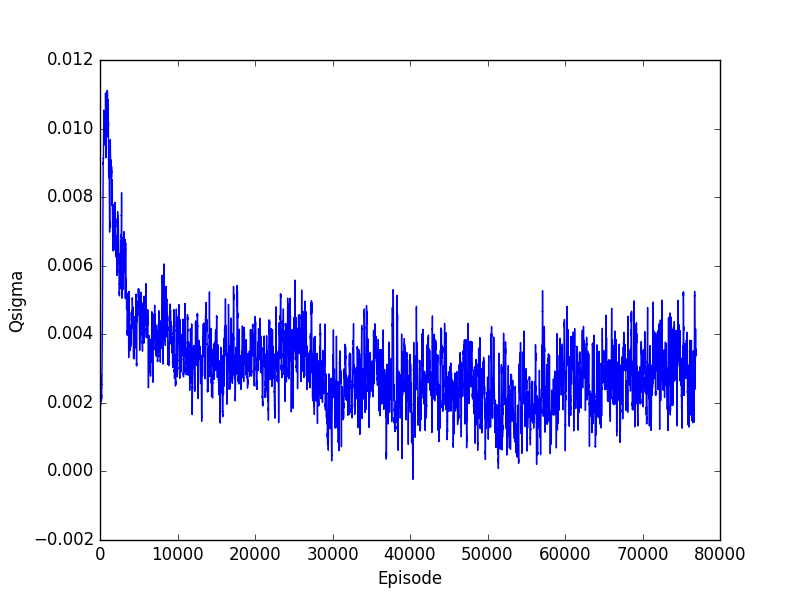
\includegraphics[width=1\textwidth]{pics/5x5_exp_Qsigma.png}
  \caption{Scores for the 5x5 opening board learned using joint distribution backup. The scores close to 1 are in fact the only winning moves.}
  \label{fig:5x5_1}
\end{subfigure}\hfill
\begin{subfigure}[t]{.45\textwidth}
  \centering
      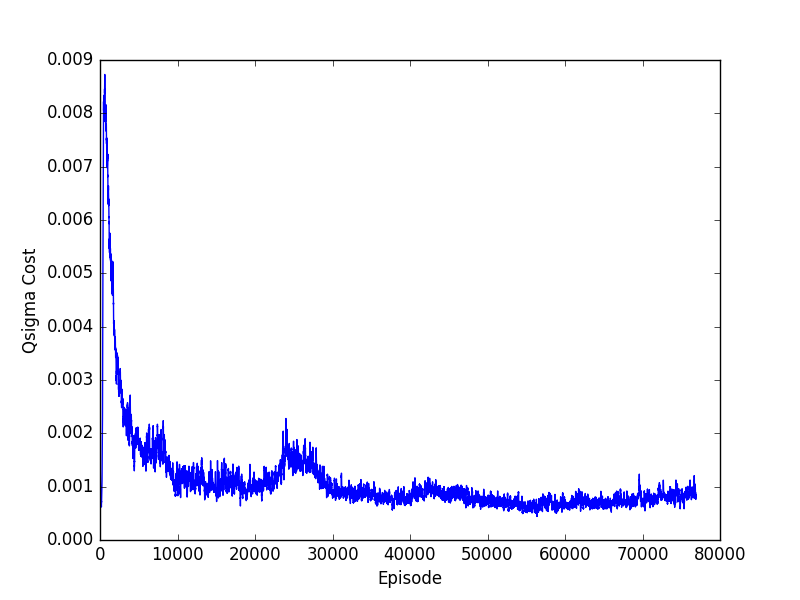
\includegraphics[width=1\textwidth]{pics/5x5_exp_Qsigma_cost.png}
  \caption{2 moves in, scores are still reasonable.}
  \label{fig:5x5_2}
\end{subfigure}
\caption{Expamples of 5x5 hexs scores learned by joint distribution backup rule. It scales very poorly to larger boards, but here it is adequate. Note, values  apparently greater than 1 are actually near 0 but the exponent was truncated.}
\label{fig:5x5}
\end{figure}

\begin{figure}[!ht]
\centering
\begin{subfigure}[t]{.45\textwidth}
  \centering
      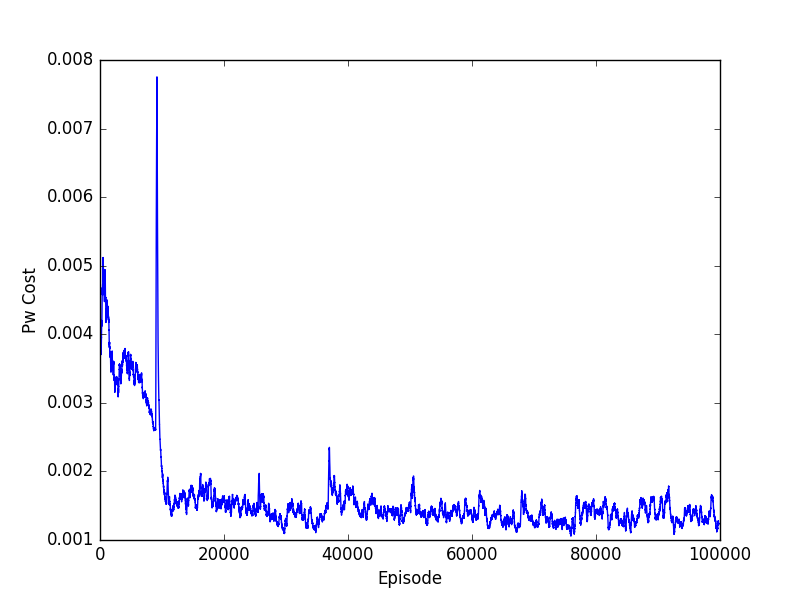
\includegraphics[width=1\textwidth]{pics/7x7_count_Pw_cost.png}
  \caption{Scores for the 5x5 opening board learned using joint distribution backup. The scores close to 1 are in fact the only winning moves.}
  \label{fig:5x5_1}
\end{subfigure}\hfill
\begin{subfigure}[t]{.45\textwidth}
  \centering
      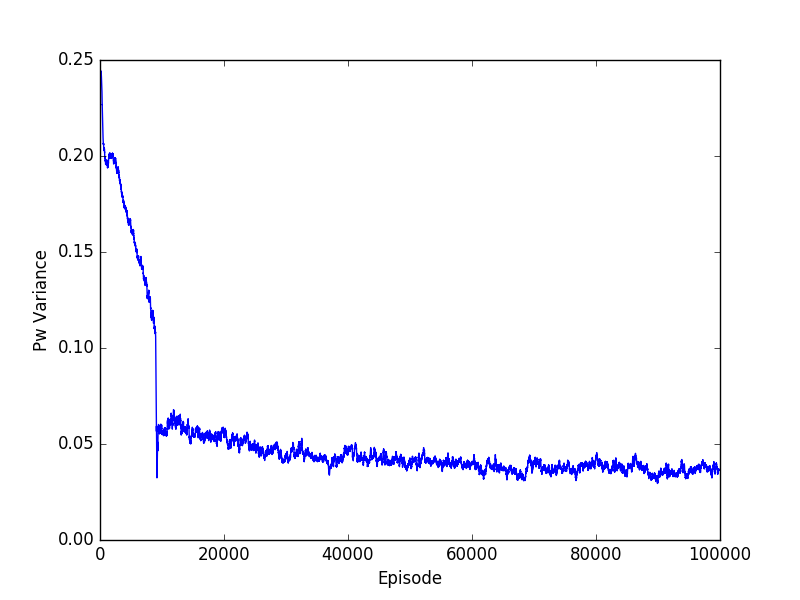
\includegraphics[width=1\textwidth]{pics/7x7_count_Pw_var.png}
  \caption{2 moves in, scores are still reasonable.}
  \label{fig:5x5_2}
\end{subfigure}\vfill
\begin{subfigure}[t]{.45\textwidth}
  \centering
      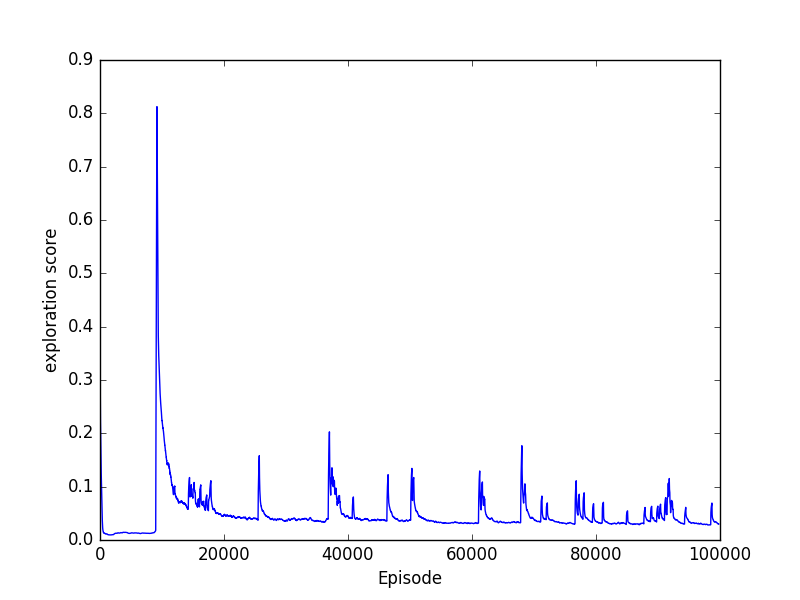
\includegraphics[width=1\textwidth]{pics/7x7_count_exp_score.png}
  \caption{Scores for the 5x5 opening board learned using joint distribution backup. The scores close to 1 are in fact the only winning moves.}
  \label{fig:5x5_1}
\end{subfigure}\hfill
\begin{subfigure}[t]{.45\textwidth}
  \centering
      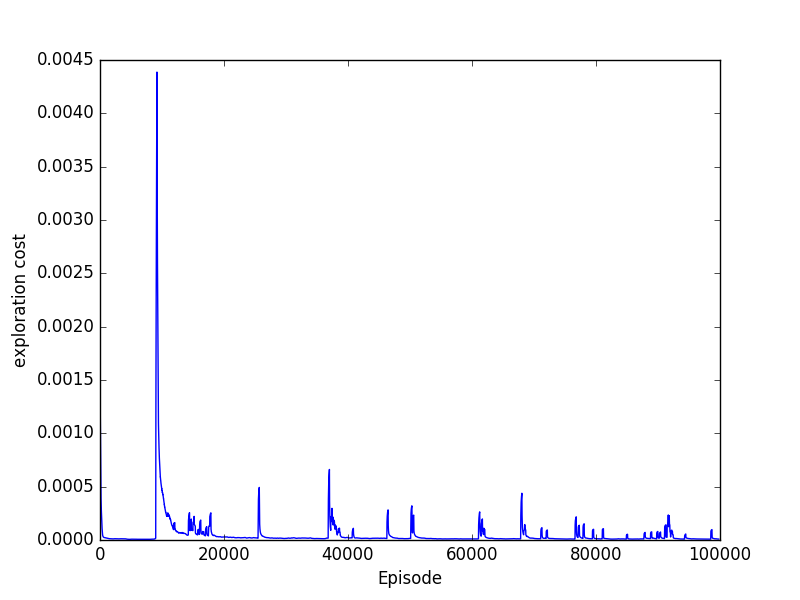
\includegraphics[width=1\textwidth]{pics/7x7_count_exp_cost.png}
  \caption{2 moves in, scores are still reasonable.}
  \label{fig:5x5_2}
\end{subfigure}\vfill
\begin{subfigure}[t]{.45\textwidth}
  \centering
      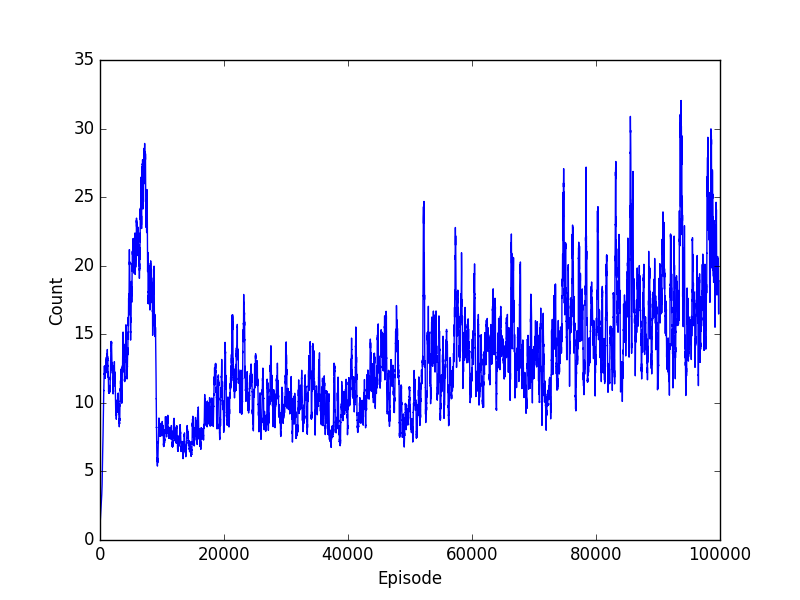
\includegraphics[width=1\textwidth]{pics/7x7_count_count.png}
  \caption{Scores for the 5x5 opening board learned using joint distribution backup. The scores close to 1 are in fact the only winning moves.}
  \label{fig:5x5_1}
\end{subfigure}\hfill
\caption{Expamples of 5x5 hexs scores learned by joint distribution backup rule. It scales very poorly to larger boards, but here it is adequate. Note, values  apparently greater than 1 are actually near 0 but the exponent was truncated.}
\label{fig:5x5}
\end{figure}

\begin{figure}[!ht]
\centering
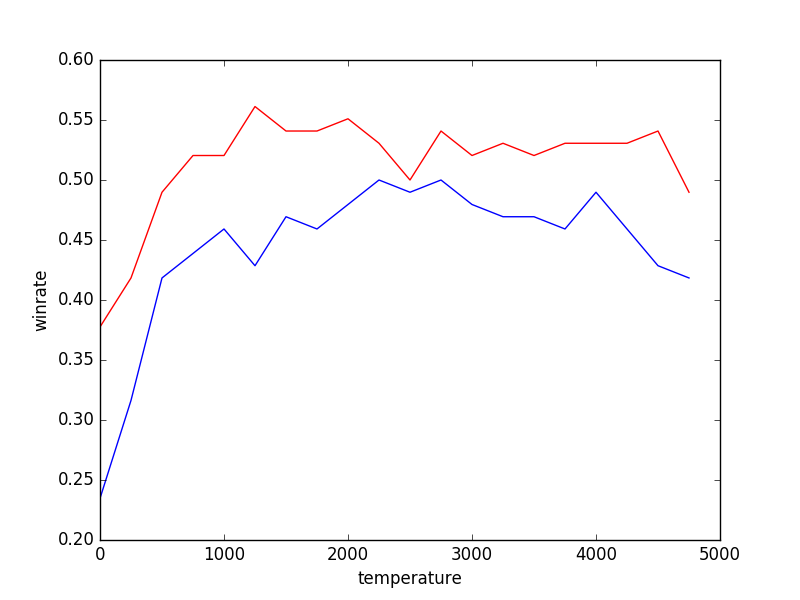
\includegraphics[width=1\textwidth]{pics/wolve_temp.png}
\caption{winrate v.s. temperature of stochastic version of wolve for normal Q-learning (red) and pseudocount Q-learning (blue).}
\end{figure}

\begin{figure}[!ht]
\centering
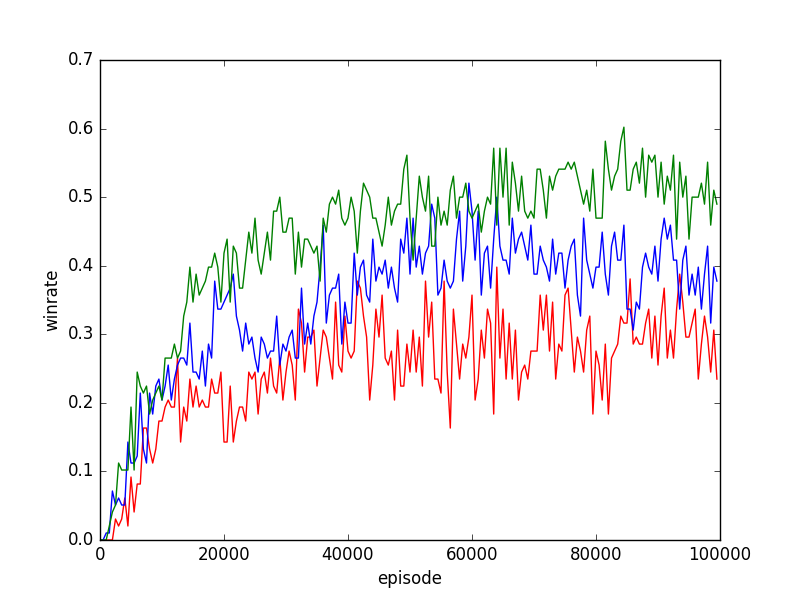
\includegraphics[width=1\textwidth]{pics/wolve_learning_curves.png}
\caption{winrate v.s. number of training episodes for normal Q-learning (green) and pseudocount Q-learning (blue) and with solver integration (red).}
\end{figure}

\section*{Conclusion}

\section*{Future Work}

\begin{thebibliography}{plain}
\bibitem{psuedocounts}
Bellemare, Marc, et al. "Unifying count-based exploration and intrinsic motivation." \textit{Advances in Neural Information Processing Systems}. 2016.
\bibitem{SCTS}
Talvitie, Erik, and FANDM EDU. "Skip context tree switching." (2014).
\bibitem{SCTS_code}
https://github.com/mgbellemare/SkipCTS
\end{thebibliography}



\end{document}